
\large Inference about $\mu_Y$ when $\sigma_Y$ is unknown (Section 5.7) \normalsize\\~\\

To use the previous Hypothesis Test or Confidence Interval for $\mu$ we need to know the true value of $\sigma^2_Y$.  In real life this is highly unlikely!\\~\\

Recall:  \underbar{~~~~~~~~~~~~~~~~~~~~~~~~~~~~~~~~~~~~~~~~~~~~~~~~~~} is the standard deviation of a statistic.  For $\bar{Y}$
$$SE(\bar{Y})=\sigma/\sqrt{n}$$
A good estimator of $\sigma$ is the sample standard deviation $S=\sqrt{\frac{1}{n-1}\sum_{i=1}^{n}(Y_i-\bar{Y})^2}$, if we plug this in for $\sigma$ we get the \\~\\~\\~\\

Our inference for $\mu$ was based on the test statistic \\~\\~\\~\\
If we plug in our estimator of $\sigma$, does \\~\\~\\~\\
\begin{center}
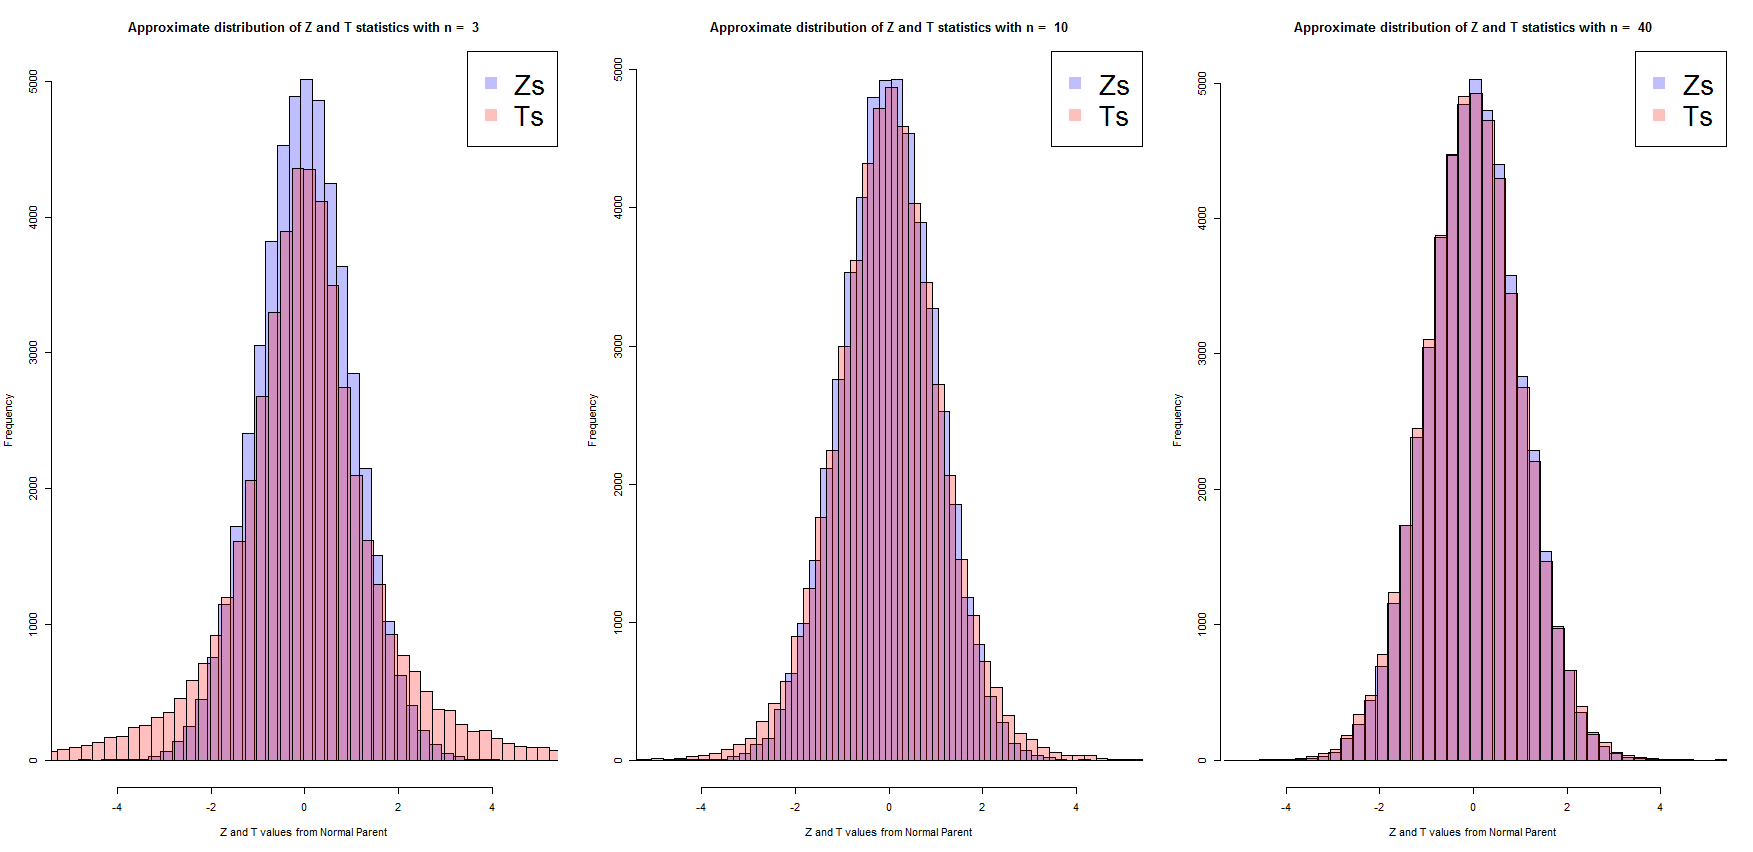
\includegraphics[scale=0.35]{zandt}
\end{center}
For data from a normal distribution
\newpage

\large T-distribution \normalsize \\~\\
t-distribution is a bell-shaped distribution centered at 0
\begin{flushright}
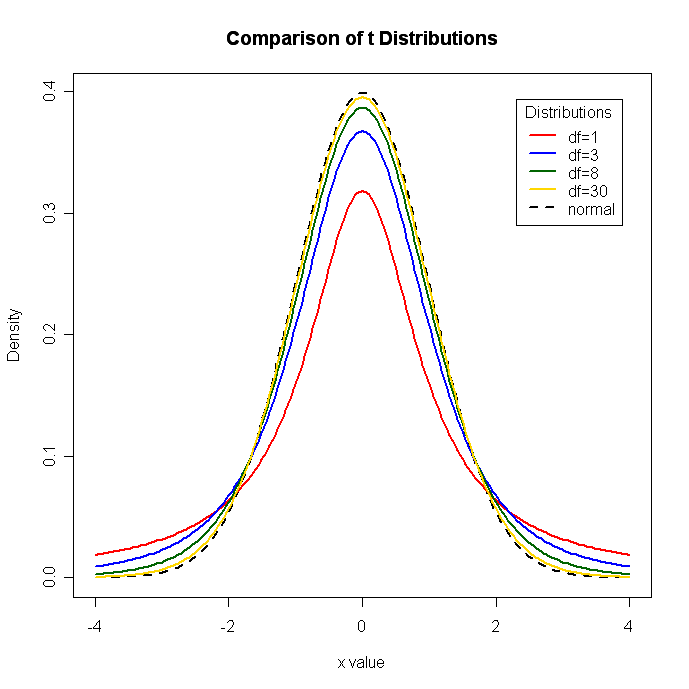
\includegraphics[scale=0.45]{tdist}
\end{flushright}

Degrees of freedom:\\~\\~\\~\\~\\

For a random sample of size $n$ where the parent population is \textit{reasonably symmetric and mound shaped}, a \large $(1-\alpha)100$\% CI for $\mu$ \normalsize is given by\\~\\~\\~\\~\\

\begin{itemize}
\item $t_{\alpha/2}$ is a multiplier from the t-dist. with $df$ = n-1 (for every df, $t_{\alpha/2}$ will be different).\\~\\~\\~\\~\\
\item Called a `one-sample t' interval for $\mu$ (our previous interval is called a `one-sample z' interval for $\mu$).
\end{itemize}

\newpage

In SAS we can get $t_{\alpha}$ or $t_{\alpha/2}$ by the following code:\\~\\
tinv(p,df) returns the pth quantile, 0$<$p$<$1, of the t distribution with df degrees of freedom.  \\
To get $t_{\alpha/2}$ we want to find the $1-\alpha/2$ quantile (or use symmetry and take the negative of the $\alpha/2$ quantile).  Thus, we can get $t_{\alpha/2}$ with the code:\\
\begin{verbatim}
data multiplier;
talpha1=tinv(1-alpha,df);
*or;
talpha2=-tinv(alpha,df);
run;
\end{verbatim}

A psychologist claims that the mean age at which children start walking is 12.5 months. Carol wants to check if this claim is true. She took a random sample of 18 children and found that the mean age at which these children started walking was 12.9 months with a standard deviation of 0.80 month. Using a 99\% Confidence Level, find a CI for $\mu$ = the true mean age at which children start walking.  Be sure to interpret the interval, state the assumptions that are met \textbf{or required} for this interval to be valid.  Can you conclude that the mean age which all children start walking is different from 12.5 months? (Helpful $T_{df}$ values - $P(T_{18}>3.55)=0.01$~~~~$P(T_{18}>3.88)=0.005$~~~~$P(T_{17}>3.57)=0.01$~~~~$P(T_{17}>3.90)=0.005$

~\\~\\~\\~\\~\\~\\~\\~\\~\\~\\~\\~\\~\\~\\~\\~\\~\\~\\~\\~\\~\\~\\~\\~\\~\\~\\~\\~\\~\\~\\~\\
For another example of a t interval for $\mu$ see example 5.17 on pg 256.

\newpage

Similarly, we can create a Hypothesis Test for $\mu_Y$ when $\sigma_Y$ is unknown.\\~\\

\large HT for $\mu_Y$ when $\sigma_Y$ is unknown \normalsize\\
Step 1/2: Setting up hypotheses - No change\\~\\
Step 3: Check Assumptions/Find Test Statistic\\~\\
Assumptions: A random sample of size $n$ where the parent population is \underbar{~~~~~~~~~~~~~~~~~~~~~~~~~~~~~~~~~~~~~~~~~~~~~~}\\~\\~\\
\underbar{~~~~~~~~~~~~~~~~~~~~~~~~~~~~~~~~~~~~~~~~~~~~~~~~~~~~~~~~~~~~~~~~~~~~~~~~~~~~~~~~~~~~~~~~~~~~~~~~~~~~~~~~~~~~~~~~~~~~~~~~~~~~~~~~~~~~~~}\\~\\%\textit{reasonably symmetric and mound shaped}
then $T=\frac{\bar{Y}-\mu_{0}}{S/\sqrt{n}}\sim t_{n-1}$ can be used as a test statistic.\\~\\~\\
Observed value of test stat - \\~\\~\\~\\
Step 4: Find RR and/or P-value - Make Decision
\\~\\~\\~\\~\\~\\~\\~\\~\\~\\~\\~\\~\\~\\~\\~\\~\\~\\~\\~\\~\\~\\~\\~\\~\\~\\~\\~\\~\\
Step 5: Interpretation - No change.
\newpage
We can get probabilities about the t distribution with a particular df using SAS via the code below:\\
\begin{verbatim}
data probs;
tprob1=probt(0.9,5); *P(T with 5 df < 0.9);
tprob2=1-probt(2.1,10); *P(T with 10 df > 2.1);
run;
\end{verbatim}

Ex:  A biology class is asked to find if the average wingspan of monarch butterflies is different from 91 mm. The class caught and measured the wingspans of 13 monarch butterflies. The average length (in millimeters) was found to be 93.5 with a standard deviation of 3.44mm. Conduct a hypothesis test with level $0.01$ using p-values.  (Use all 5 steps and be sure to state assumptions you must make for this procedure to be valid.  Also, how would you investigate that assumption based off your data set?)  $P(T_{13}>2.620)=0.0106$~~$P(T_{12}>2.620)=0.0112$~~$P(T_{13}>-2.620)=0.9894$~~$P(T_{12}>-2.620)=0.9888$~~$P(T_{90}>93.5)\approx 0$

\newpage

Note: If $n$ is `large' $(>30)$ then in practice you often use $z$ critical value (multiplier) and use the standard normal to create the RR and to find the p-value.\\~\\
Ex:  Suppose that we are interested in testing whether or not the average NCSU student spent more than \$200 this semester on textbooks.  We randomly sample 50 students and ask them how much they spent this semester on textbooks.  Suppose that the sample average was \$204.5 and the sample standard deviation was \$20.12.  Carry out a hypothesis test using the RR approach with $\alpha=0.02$. Useful values: $P(T_{49}>1.68)=0.05$~~~~$P(T_{49}>2.40)=0.01$~~~~$P(T_{49}>2.01)=0.025$~~~~$P(T_{49}>2.11)=0.02$\\~\\
Steps 1/2: $\mu=$ (true) average amount spent on textbooks this semester for NCSU students\\
$$H_0: \mu = 200~~~~or~~~~H_0: \mu \leq 200$$
$$H_A: \mu > 200$$
Step 3: Since RS and n is large we can use 
$$T=\frac{\bar{Y}-\mu_{0}}{S/\sqrt{n}}\sim t_{n-1}$$ 
as our test statistic.
$$t_{obs}=\frac{\bar{y}-\mu_{0}}{s/\sqrt{n}}=\frac{204.5-200}{20.12/\sqrt{50}}=1.582$$
Step 4: RR determined by the alternative hypothesis and our test statistic.  Since $T\sim t_{n-1}$ and we have a `$>$' alternative our RR is 
$$RR=\left\{t_{obs}:t_{obs}>2.11\right\}$$
Since $1.582<2.11$ we fail to reject $H_0$.\\~\\
Step 5: At the 2\% significance level, there is not enough evidence to support the alternative that the true average amount spend on textbooks this semester by NCSU students is greater than \$200.\\~\\
Note:  If we had used a standard normal instead of the $t_{49}$ our RR would have been 
$$RR=\left\{t_{obs}:t_{obs}>2.05\right\}$$
This is pretty close, and so often for very large $n$ we simply use the standard normal distribution instead of the $t$.
\\~\\~\\~\\~\\~\\~\\~\\~\\~\\~\\~\\
For another HT using the t, see example 5.15 on pg 253.




